\documentclass[8pt]{beamer}
\usepackage[utf8]{inputenc}
\usepackage{xcolor}
\usepackage{graphicx}
\usepackage{colortbl}
\usepackage{epsfig}
% \usepackage{cancel}
\usepackage{ulem}
% \usepackage{threeparttable} % Joao Pela: 
\usepackage{amsmath}
\usepackage{hyperref}
\usepackage{appendixnumberbeamer}
\usepackage{feynmp}         % For latex produced Feynman Diagrams

\newcommand\Fontvi{\fontsize{6}{7.2}\selectfont}

\newcommand{\totlumi}{19.6~fb$^{-1}$}
\newcommand{\pta}{p_{\rm T}^{\rm j1}}
\newcommand{\ptb}{p_{\rm T}^{\rm j2}}
\newcommand{\etaa}{\eta_{\rm j1}}
\newcommand{\etab}{\eta_{\rm j2}}
\newcommand{\sgneta}{\etaa \cdot \etab}
\newcommand{\etajj}{\Delta \eta_{\rm jj}}
\newcommand{\phijj}{\Delta \phi_{\rm jj}}
\newcommand{\mjj}{M_{\rm jj}}
\newcommand{\met}{\displaystyle{\not} E_{\rm T}}
\newcommand{\W}{{\rm W}}
\newcommand{\Z}{{\rm Z}}
\newcommand{\stat}{\text{ (stat.)}}
\newcommand{\syst}{\text{ (syst.)}}

\usetheme{Madrid}

\author[J. Pela]{João Pela, on behalf of the CMS Collaboration}
\title[Search for VBF Higgs $\rightarrow$ Inv at CMS]{Search for invisible Higgs decays in the VBF channel using the CMS detector}
\institute[ICL]{Imperial College London}
\date{2014-04-07}

% The log drawn in the upper right corner.
\logo{\includegraphics[height=0.115\paperheight]{img/Logo_CMSICL.png}}

\begin{document}
\setlength{\unitlength}{1mm}

% ###################################################
\begin{frame}
  \titlepage
\end{frame}

% ###################################################
\begin{frame}{Introduction}
\Fontvi
 
\begin{block}{SM Higgs boson compatibility}
 
All measurements of the 125 GeV boson to date indicate compatibility with a SM Higgs boson, but:
\begin{itemize}
 \item associated uncertainties are large
 \item the possibility for non-SM properties remains
\end{itemize}

Additional SM-like Higgs bosons have been excluded over a wide mass range, additional Higgs bosons with exotic decay modes remains a possibility, and are predicted by many models.

\end{block}

\begin{block}{BSM invisible Higgs boson decay modes:}

\begin{itemize}
 \item Neutralinos in supersymmetric models.
 \item Graviscalars in models with extra dimensions. 
\end{itemize}

\end{block}

\begin{block}{Indirect measurements}

The ATLAS and CMS collaborations have used the visible decay modes to infer limits on the invisible branching fraction of the 125 GeV Higgs boson:
\begin{itemize}
 \item ATLAS: upper limit of 60\%
 \item CMS: upper limit limit is 64\%
\end{itemize}

\end{block}

\begin{block}{Motivations direct searches for invisible decays:}

\begin{itemize}
 \item Observation of a signal in such searches would be a \uline{clear indication} of physics beyond the SM.
 \item Non-observation provides the opportunity to further \uline{constrain the properties} of the newly discovered boson.
\end{itemize}

\end{block}
 
\end{frame}

% ###################################################
\begin{frame}{VBF Channel}

\begin{columns}
 
\column[t]{0.45\linewidth}
\begin{block}{Direct searches channels}

On direct searches rely on associated production modes, where the Higgs recoils against a visible system.
\begin{itemize}
 \item Z Associated production: Low production cross section; Clear final state, but low sensitivity with the available data.
 \item VBF mode: Substantially higher cross section. Shown to offer greater sensitivity to invisible decays.
\end{itemize}

\end{block}

\begin{block}{VBF Higgs Diagram}
 
\centering
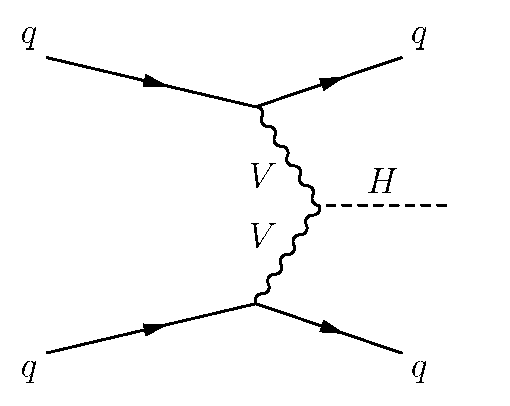
\includegraphics[width=0.45\linewidth]{img/feyn_VBF.pdf} 

\end{block}

\column[t]{0.45\linewidth}
\begin{block}{VBF Higgs to invisible search}

Search for final states with:
\begin{itemize}
 \item two jets and large missing energy
 \item use the distinct topology of the VBF jets to distinguish invisible Higgs decays from background
\end{itemize}
 
\end{block}

\begin{block}{Backgrounds}

Major:
\begin{itemize}
 \item $Z \rightarrow \nu \nu$, in association with jets
 \item $W \rightarrow l \nu$, with charged lepton misidentified
\end{itemize}

Minor:
\begin{itemize}
 \item Mismeasurement of QCD events
 \item Other SM processes
\end{itemize}

\end{block}

\end{columns}

\end{frame}

% ###################################################
\begin{frame}{Analysis Definition}
 
\begin{block}{Dedicated trigger}
 
\begin{itemize}
 \item Any forward/backward pair of jets satisfying:
 \begin{itemize}
  \item pair of jets $p_t>40 GeV$
  \item $\Delta\eta_{jj} = | \eta_{jet1} - \eta_{jet2}| > 3.5$
  \item High invariant mass ($m_{jj}>800$ GeV)
 \end{itemize}
 \item $MET>65$ GeV
\end{itemize}
 
\end{block}

\begin{block}{Offline selection}
 
\begin{itemize}
 \item Standard MET filters: remove anomalous calorimeter signals, beam halo, calorimeter laser calibration events and tracking failure. 
 \item Good vertex: ($|z|<24$ cm, $r<2$ cm) and $+10$ tracks
 \item $e/\mu$ veto: electron or muon with $p_t>10$ GeV
 
 \item Dijet: leading PF AK5 jet pair that pass pile-up jet rejection:
 \begin{itemize}
  \item $\eta_{jet1} . \eta_{jet2} < 0$
  \item $p_t > 50$ GeV, $\eta < 4.7$
  \item $m_{jj}>1100$ GeV
  \item $\Delta\phi_{jj} < 1.0$
 \end{itemize}

 \item $PF_{MET} > 130$ GeV
 
 \item Central Jet Veto (CJV): Veto if any jet at $\eta_{jet1} < \eta < \eta_{jet2}$ and $p_t>30$ GeV
 
\end{itemize}
 
 
\end{block}
 
\end{frame}

% ###################################################
\begin{frame}{Background Estimation Methods I}
\Fontvi 
 
\begin{block}{$\Z (\rightarrow \nu \nu)+$jets}

Estimated from data using observable $\Z \rightarrow \mu \mu$ decays:

\begin{itemize}
 \item Identical selection for signal region except lepton veto is replaced with a $\Z \rightarrow \mu \mu$ requirement.
 \item reconstructed muons with $p_t > 20 $ GeV, and $60 < M_{\mu\mu}<120$ GeV, 
 \item veto on additional leptons, 
 \item $\met$ recomputed after removing the \Z muons.  
 \item We use MC to extrapolate obtained control region yield to background contribution of this channel in the signal region
\end{itemize}

\end{block}
 
\begin{block}{$\W (\rightarrow \ell \nu)+$jets}

For $\W \rightarrow {\rm e} \nu$ and $\W \rightarrow \mu \nu$ 
\begin{itemize}
 \item Same method as $\Z (\rightarrow \nu \nu)+$jets
 \item Remove lepton veto and require a single charged lepton ($e/\mu$)
 \item Veto additional leptons
 \item $\met$ is recomputed after removing the W muon (not for the electron since was included on trigger)
\end{itemize}

For $\W \rightarrow \tau\nu$ where the tau decays hadronically
\begin{itemize}
 \item Control region is defined in the same way as $\W \rightarrow \ell \nu$
 \item Required one hadronic tau, no additional leptons
 \item The central jet veto is not applied in order to increase the yield
\end{itemize}

Again for all $\W (\rightarrow \ell \nu)+$jets we using MC to extrapolate control region yield to background contribution of this channel in the signal region

\end{block} 
 
\end{frame}

% ###################################################
\begin{frame}{Background Estimation Methods II}

\begin{block}{QCD Multijets}

Use the fractions of events passing the $\met$ and CJV cuts, after the full remaining selection. We define regions ABCD as follows:

\begin{itemize}
 \item{A : fail $\met$, fail CJV}
 \item{B : pass $\met$, fail CJV}
 \item{C : fail $\met$, pass CJV}
 \item{D : pass $\met$, pass CJV}
\end{itemize}

We estimate the QCD multijet component in regions ABC by subtracting MC electroweak backgrounds from data. We then estimate the QCD multijet component in the signal region D, to be $D = BC / A$

\end{block}

\begin{block}{Other backgrounds}
 
All other minor backgrounds were estimated from MC.
 
\end{block}
 
\end{frame}

% ###################################################
\begin{frame}{Event Yield and Bkg. Estimation}

The results of the background estimation are summarised here:

\begin{block}{Yields}

\begin{table}[th!]
\centering
% \caption{Summary of estimated backgrounds and observed yield in the signal region.}
\begin{tabular}{|l|c|}
\hline
Background 	 		& $N_{\rm est}$ \\
\hline
$Z \rightarrow \nu\nu$ 		& $102 \pm 30 \stat \pm 26 \syst$	\\
$W \rightarrow \mu\nu$ 	 	& $67.2 \pm 5.0 \stat \pm 15.1 \syst$ 	\\
$W \rightarrow {\rm e} \nu$  	& $68.2 \pm 9.2 \stat \pm 18.1 \syst$	\\
$W \rightarrow \tau \nu$ 	& $54 \pm 16 \stat \pm 18 \syst$ \\
QCD multijet 	 		& $36.8 \pm 5.6 \stat \pm 30.6 \syst$ \\
Other SM			& $10.4 \pm 3.1 \syst$ \\
\hline
Total background		& $339 \pm 36 \stat \pm 50 \syst$  \\
Observed 			& $390$  \\	
\hline
\end{tabular}
\end{table}

\end{block}

Assuming a 125 GeV Higgs with 100\% invisible branching fraction, produced via VBF with the SM production cross-section, the expected yield is 208 events. In the signal region in data, we observe 390 events, which is \uline{compatible with the background prediction}.

\end{frame}

% ###################################################
\begin{frame}{Limits on invisible Higgs}
 
Assuming a background-only hypothesis, we place upper limits on an invisible Higgs signal.  
\begin{itemize}
 \item Calculated to 95\% C.L. with an asymptotic ${\rm CL}_{\rm S}$ method
 \item Using the standard CMS Higgs combination technique
\end{itemize}
 
\begin{columns}
 
\column[t]{0.45\linewidth}
\begin{block}
 
\centering
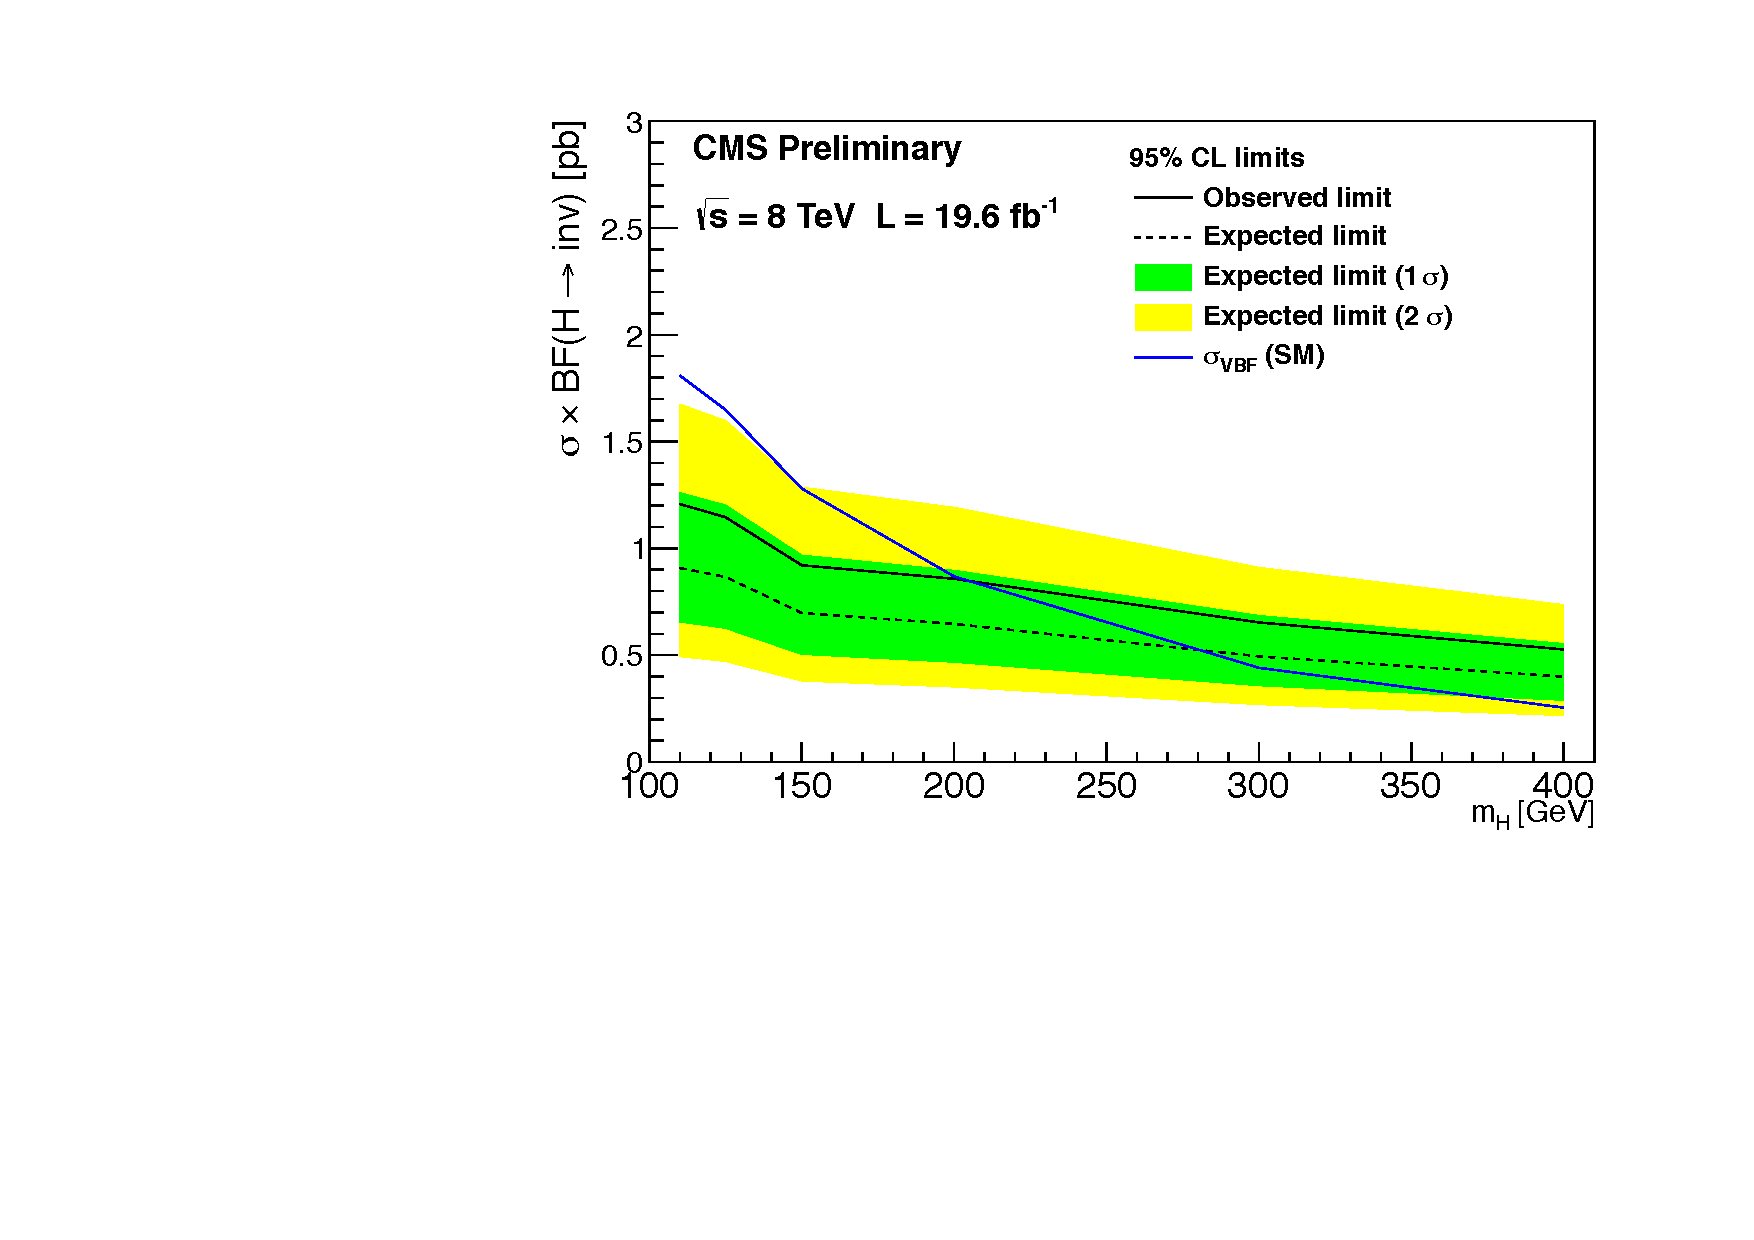
\includegraphics[width=\linewidth]{img/XSLimit.pdf} 

\end{block}

\column[t]{0.45\linewidth}
\begin{block}
 
\centering
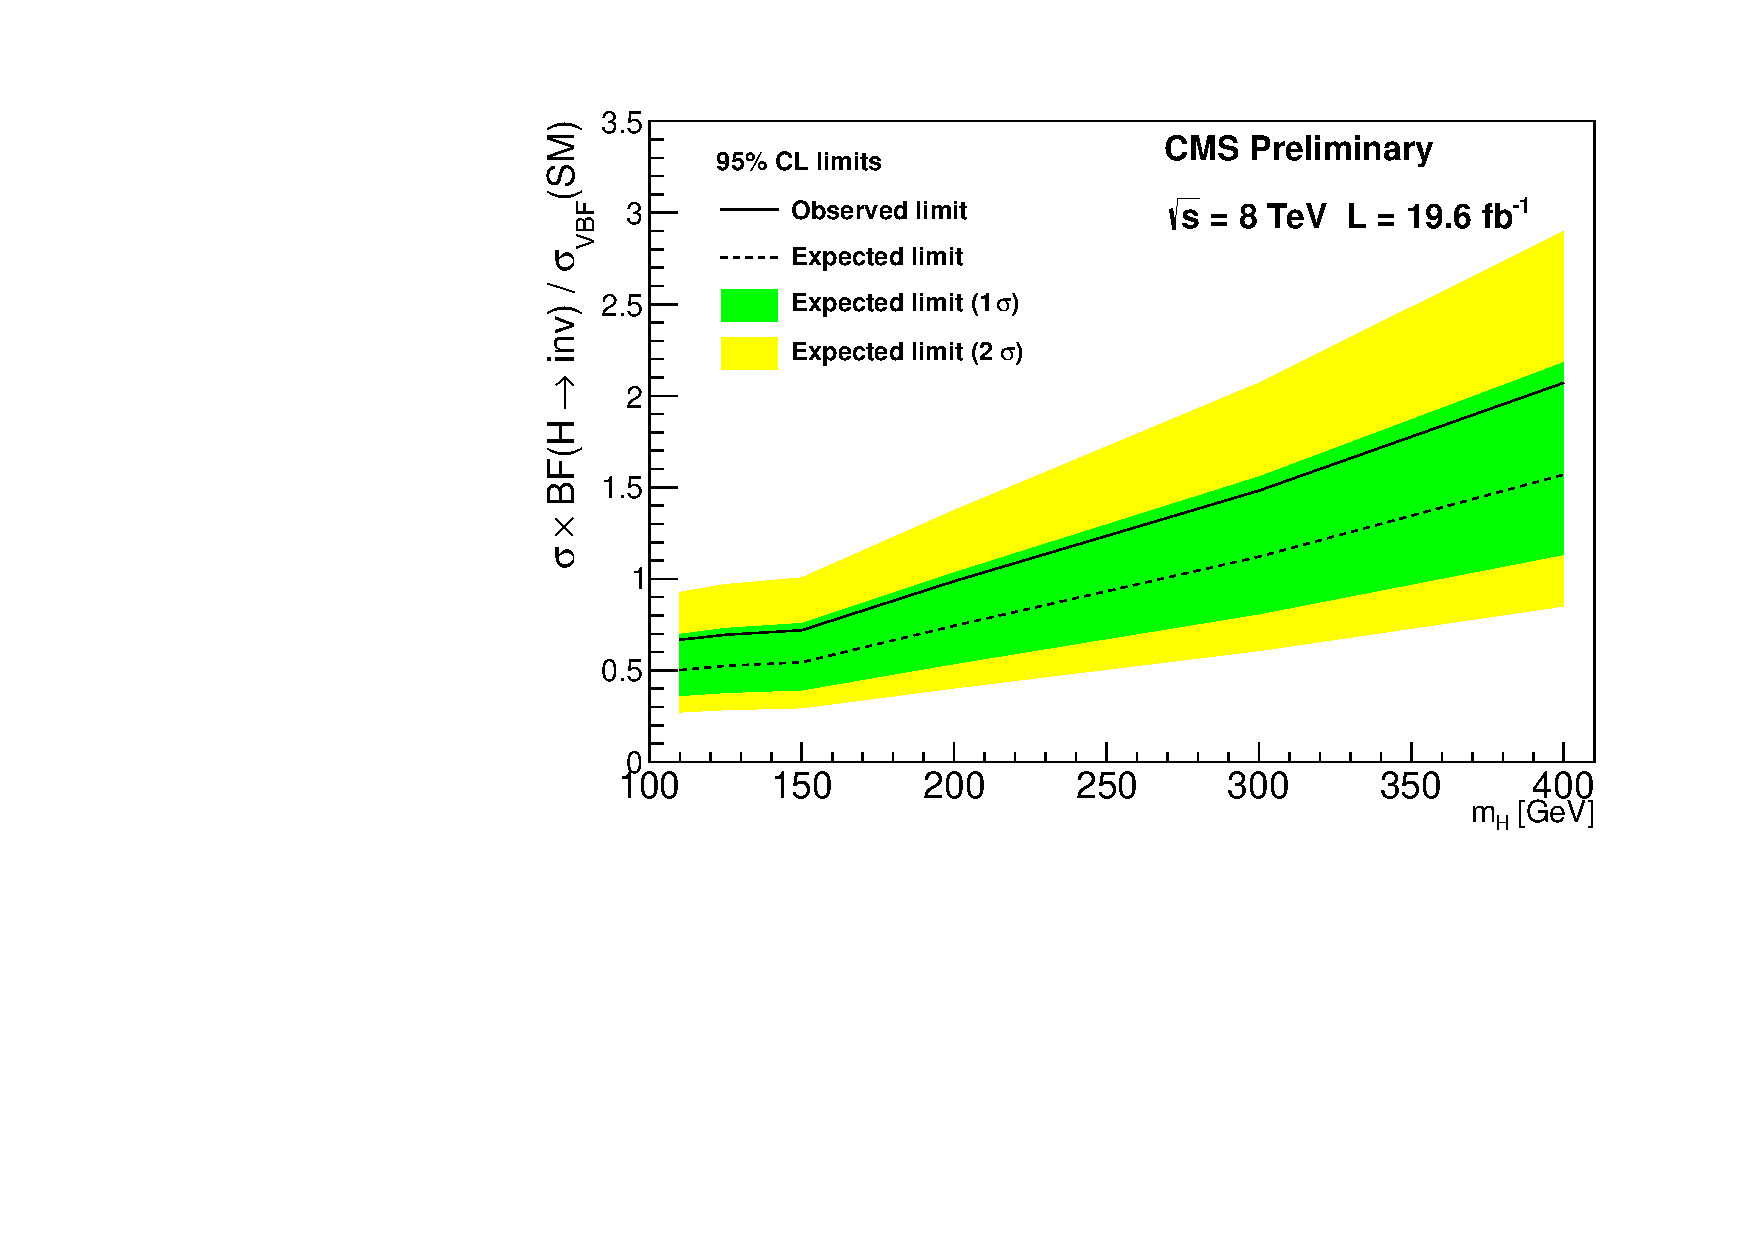
\includegraphics[width=\linewidth]{img/xsiLimit.pdf} 

\end{block}

\end{columns}

\begin{itemize}
 \item On the left, observed and expected limits on the production cross-section times invisible branching fraction as a function of the Higgs mass. 
 \item On the right, the same limits, normalised to the SM VBF production cross section.
\end{itemize}

Assuming the SM VBF production cross section, the observed limit on the invisible branching fraction of the 125 GeV Higgs 69\% and the expected limit is 53\%. 

\end{frame}

% ###################################################
\begin{frame}{Combining VBF Inv. and ZH}
 
Our results were combined with the ones from $ZH, (Z \rightarrow \ell\ell)$  analysis to obtain further sensitivity.
 
\begin{columns}
 
\column[t]{0.45\linewidth}
\begin{block}{VBF Higgs Diagram}
 
\centering
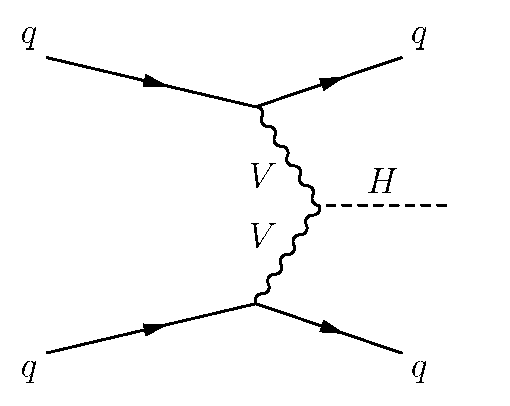
\includegraphics[width=0.8\linewidth]{img/feyn_VBF.pdf} 

\end{block}

\column[t]{0.45\linewidth}
\begin{block}{ZH Diagram}
 
\centering
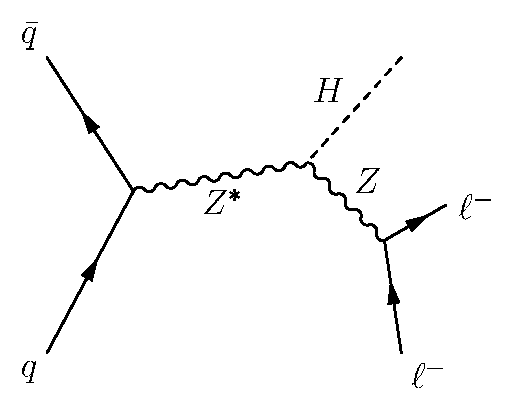
\includegraphics[width=0.8\linewidth]{img/feyn_Zll.pdf} 

\end{block}

\end{columns}

We used recently published results from CMS analysis  HIG-13-018 which reported an upper limits on the invisible branching fraction of a 125 GeV Higgs of 75\%.

\end{frame}

% ###################################################
\begin{frame}{Combination Results}
  
\begin{columns}
 
\column[t]{0.45\linewidth}
\begin{block}{Combined Limits on invisible Higgs}
 
\centering
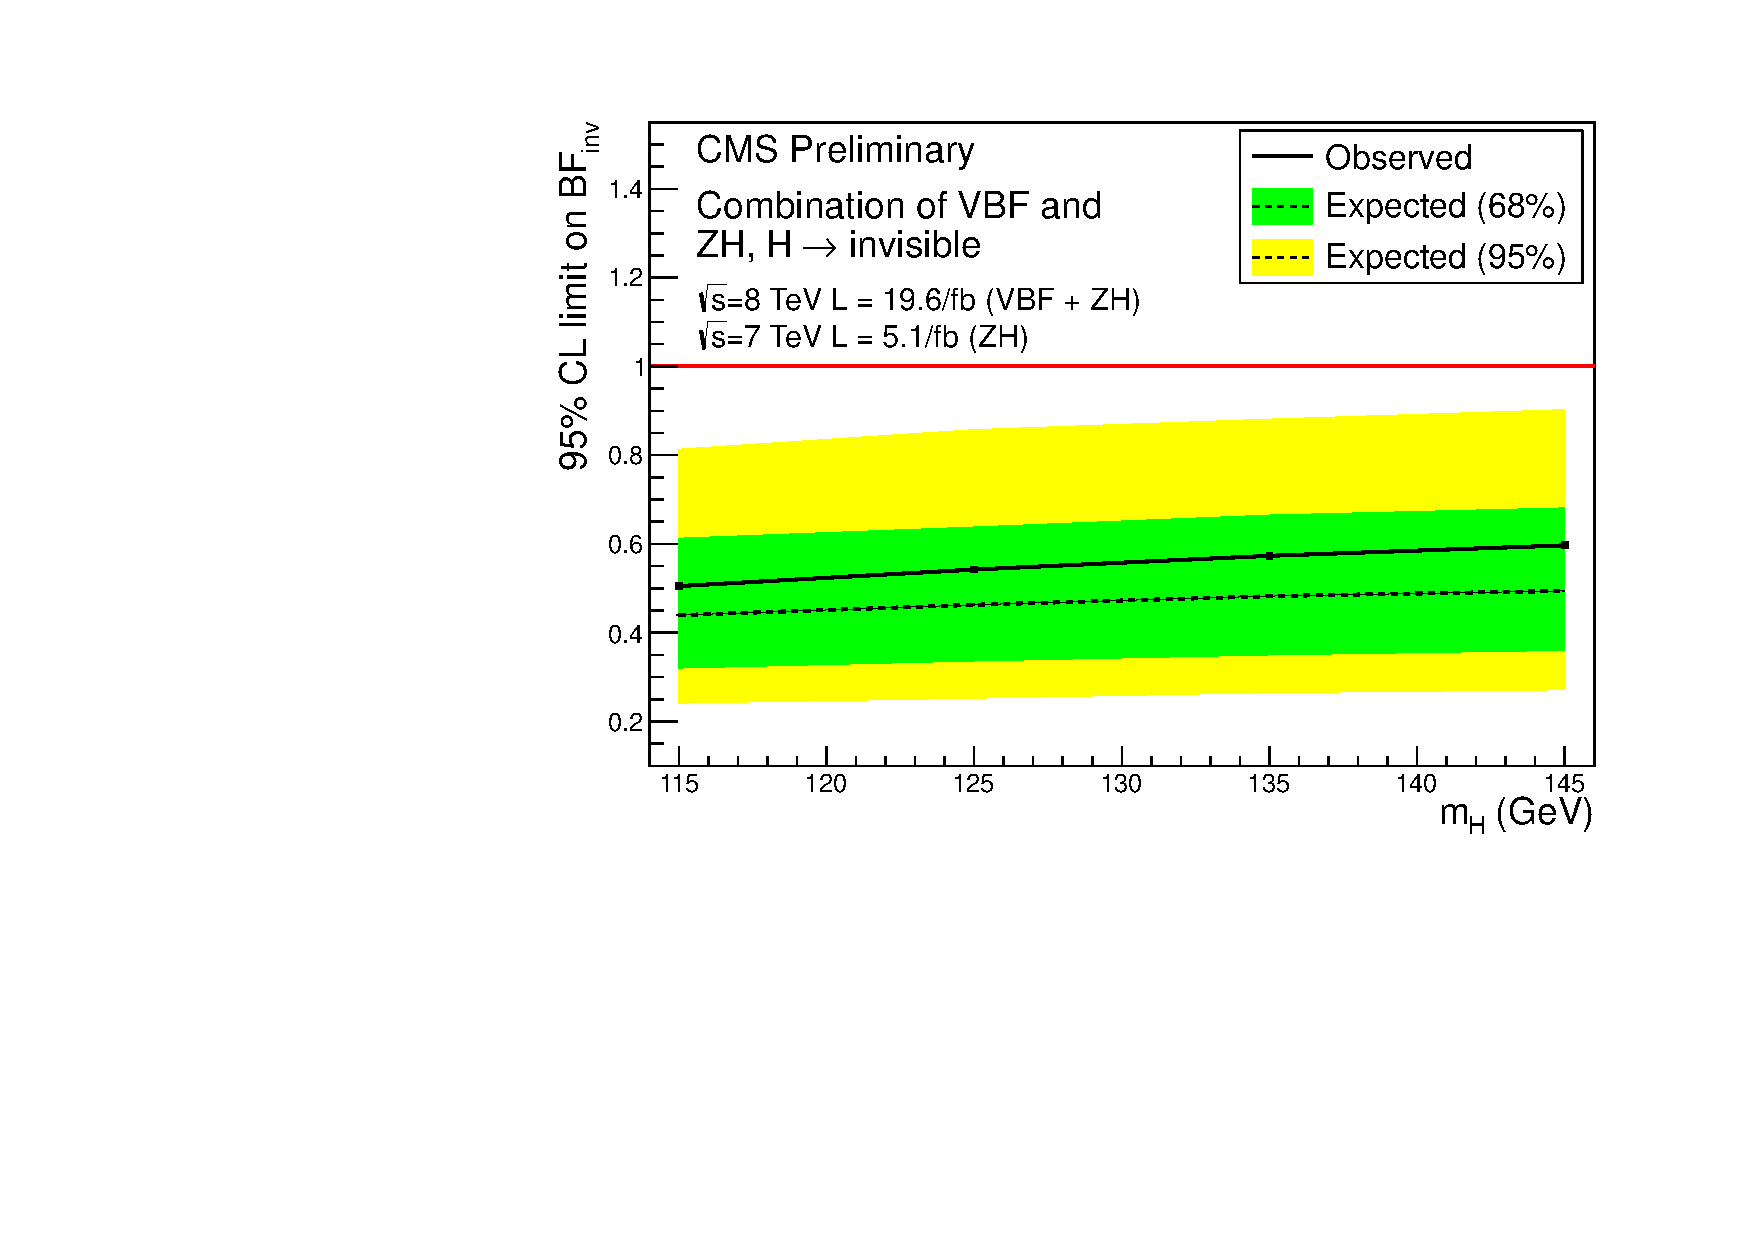
\includegraphics[width=\linewidth]{img/invlimitfinal.pdf} 

\end{block}

\column[t]{0.45\linewidth}
\begin{block}

\begin{itemize}
 \item 95\% CL upper limit on the branching fraction of a Higgs boson to invisible final states as a function of the Higgs boson mass
 \item SM production cross-sections for the Higgs boson have been assumed
 \item For a Higgs boson mass of 125 GeV the observed (expected) upper limit on the invisible branching fraction is 54 (46)\%
 \item Systematic errors between analysis considered uncorrelated
 \item New combination result including $ZH, (Z \rightarrow b\bar{b})$ under final stages of approval/publication. 
\end{itemize}
 
\end{block}

\end{columns}
 
\end{frame}

% ###################################################
\begin{frame}{Summary}

\begin{block}

\begin{itemize}
 \item A search for an invisibly decaying Higgs boson produced via vector boson fusion has been performed. 
 \item The analysis used of a dedicated trigger and offline selection to isolate events with significant missing energy and two jets with vector boson fusion characteristics
 \item Major background estimated using data driven methods.  
 \item Using the full $\sqrt{s}=8$ TeV dataset recorded by CMS in 2012, a total of $339 \pm 36 \stat \pm 50 \syst$ events are expected in the signal region, from a background only hypothesis.  
 \item Assuming a 125 GeV Higgs produced via vector boson fusion, with 100\% invisible branching fraction, would be expected to yield 208 events. Yet observe 390 events in the signal region in data, which compatible with the expected background.
 \item Using an asymptotic ${\rm CL}_{\rm S}$ method, 95\% CL upper limits are placed on the production cross section times invisible branching fraction.  The observed limit on the invisible branching fraction of the 125 GeV Higgs is 69\%, with an expected limit of 53\%.  
 \item This measurement is the most sensitive to invisible decays of the Higgs boson to date.
 \item Combination with $ZH, (Z \rightarrow b\bar{b})$ is presented and the obtained observed (expected) upper limit on the invisible branching fraction is 54 (46)\%
\end{itemize}

\end{block}

\end{frame}

% ###################################################
\appendix
% ###################################################
\begin{frame}
 
\begin{block}

\begin{center}Backup Slides\end{center}

\end{block}

\end{frame}

\end{document}